\section{About Monetary Economics}

Does an unanticipated shock to money affect real side of the
economy (quantities)?

\begin{itemize}
    \item Classical view: If prices are flexible, the shock
    will change wages and prices proportionally, but not change the quantities.

    If the gov prints money and spend it, the prices increase and nominal assets lose in value, 
    which is negative wealth effect.

    Money supply increase acts like a tax on nominal asset 
    holdings, some call it 'inflation tax'.

    \item Keynesian view: Prices are rigid, so the shock will
    give a positive wealth effect, this assumes that new money is distributed proportionally to existing money holdings.
\end{itemize}

How should we conduct monetary policy?

\begin{itemize}
    \item Monetatists: steady money supply growth, in line with money
    demand growth.
    \item Keynesians: use expansionary MP to stimulate the economy
    in a recession.
    \item Inflation of 70's and subsequent successful tight MP(Volcker)
    led to Monetarists becoming very influential.
\end{itemize}

\section{Lucas Critique}

The Lucas critique (Lucas 1976\cite{lucas1976econometric}) is an important philosophical point that forms the basis of much
of modern macroeconomics.
From Keynes until the mid-1970s, macroeconomics looked very different
to what it does now.

\underline{\textcolor{blue}{\textbf{Theoretical side:}}}
\begin{itemize}
    \item used variants of a textbook IS-LM (investment-
    saving liquidity-money) model: not take agent optimisation, dynamics, or expectations
    formation very seriously
\end{itemize}

\underline{\textcolor{blue}{\textbf{Empirical side:}}}
\begin{itemize}
    \item used large-scale macroeconometric models, systems of simultaneous equations featuring aggregate variables – many of the
    larger models would feature hundreds of variables
\end{itemize}

The design of these macroeconometric models was based on fit and forecasting - regressions, essentially - with little attention paid to any underlying
theory or actual economics. There was no microfoundation, and agents' behaviour was postulated to
be based on adaptive expectations, which were essentially ad-hoc.

The essential gist of Lucas' Critique is that it is fraught with hazard to try and predict the effects
of a policy change based on correlations (regression coefficients) based on historical data.

\subsection{Is econometrics useful?}

The conclusion of the Lucas Critique is that we need to take economic theory seriously – correlations
(or regression coefficients) estimated in the data may not be policy-invariant, and therefore may not
be useful in thinking about “counterfactuals” where we think of what would happen under alternative
policy regimes.

The Lucas Critique tells us that we need to take theory seriously when
doing econometrics; and when we do econometrics without theory (e.g. reduced form econometrics), be
honest and open about the potential misgivings.

\subsection{Empirical evidence on the effects of money supply shocks}

\underline{\textbf{Problem with identification of Monetary Policy: reverse causality.}}

The most widly accepted econometric methodology is the VAR (Vector Autoregression) model.

\begin{eg}
    \ 

    Example with detrended money stock $M$ and detrended real output $Y$:
    \begin{align*}
        Y_t &= \phi_{YY}Y_{t-1} + \phi _{YM}M_{t} + u_{t}^Y \\ 
        M_t &= \phi_{MY}Y_{t} + \phi _{MM}M_{t-1} + u_{t}^M
    \end{align*}
    where $u^M$ are money supply shocks and $u^Y$ are output supply(e.g. TFP) shocks(independent from other time $t$ variables and from each other).
\end{eg}

Then we consider another simple example:
\begin{eg}
    \begin{align*}
        Y_t &= \phi_1 Y_{t-1} + \phi_2 M_{t} + \phi_3 M_{t-1} + u_{t}^Y \\ 
        M_t &= \phi_4 Y_{t} + \phi_5 M_{t-1} + \phi_6 Y_{t-1} + u_{t}^M
    \end{align*}
    The problem is: OLS will provide inconsistent estimate of $\phi$.
    We could do it if we have direct measures of the shocks, or an instrument(but we don't).

    We rearrange the equations to get:
    \begin{align*}
        Y_t &= \frac{1}{1 - \phi_2 \phi_4} \left( (\phi_1 + \phi_2 \phi_6)Y_{t-1} + (\phi_3 + \phi_2 \phi_5)M_{t-1} + u_t^Y + \phi_2 u_t^M \right) \\
        M_t &= \frac{1}{1 - \phi_2 \phi_4} \left( (\phi_6 + \phi_4 \phi_1)Y_{t-1} + (\phi_5 + \phi_4 \phi_3)M_{t-1} + u_t^M + \phi_4 u_t^Y \right)
    \end{align*}
    Now, we can run OLS estimation! THis gives us consistent estimatess of coefficients(under the assumption that $u$ are $\perp$ to variables at $t-1$.)
    
    Still, we estimate 4 coefficients, and have 6 unknowns.

    Residuals we get are:
    \begin{align*}
        \varepsilon_t^Y &= \frac{1}{1-\phi_2 \phi_4} (u_t^Y + \phi_2 u_t^M) \\
        \varepsilon_t^M &= \frac{1}{1-\phi_2 \phi_4} (u_t^M + \phi_4 u_t^Y)
    \end{align*}
    Then, we need to make additional identifying assumptions! Currently, there are two alternatives:
    \begin{enumerate}
        \item $\phi_4 = 0$, monetary policy does not react to the
        contemporaneous level of output.
        \[\varepsilon_t^Y = \phi_2 \varepsilon_t^M + \frac{1}{1-\phi_2 \phi_4} u_t^Y\]
        We can estimate $\phi_2$ from regression of $\varepsilon_t^Y$ on $\varepsilon_t^M$.
        \item $\phi_2 = 0$, output does not react to change in monetary policy.
        We can estimate $\phi_4$ from regression of $\varepsilon_t^M$ on $\varepsilon_t^Y$.
    \end{enumerate}
    Either assumption identifies all the parameters of the VAR.

    Once we have all the $\phi$ parameters, we know the economy's response to a money shock 
    $u_t^M$ or to a real shock $u_t^Y$.
\end{eg}

\subsubsection{Technical aside: Granger causality}

Granger(1969\cite{granger1969investigating}) introduced the concept of Granger causality based on forecasting techniques 
in time series econometrics. A variable $X$ is said to Granger-cause $Y$ if and only if 
lagged values of $X$ have marginal predictive content in a forecasting equation for $Y$.
In other words, having some information about the future of $Y$ is not enough for Granger causality, 
and that past observations of $X$ should have more information about
the future of $Y$ than the past $Y$ observations.

Consider the simple bivariate VAR(2) model:
\begin{align*}
    Y_{1,t} &= c_1 + \phi_{11}^{(1)} Y_{1,t-1} + \phi_{12}^{(1)} Y_{2,t-1} + \phi_{11}^{(2)} Y_{1,t-2} + \phi_{12}^{(2)} Y_{2,t-2} + \epsilon_{1,t}, \\
    Y_{2,t} &= c_2 + \phi_{21}^{(1)} Y_{1,t-1} + \phi_{22}^{(1)} Y_{2,t-1} + \phi_{21}^{(2)} Y_{1,t-2} + \phi_{22}^{(2)} Y_{2,t-2} + \epsilon_{2,t}.
\end{align*}

$Y_2$ does not Granger-cause $Y_1$ is analogous to saying that the coefficients of $Y_2$ in the $Y_1$ equation are all 0. 
In other words, $\phi_{12}^{(1)} = \phi_{12}^{(2)} = 0$. We can test for the Granger causality running from $Y_2$ to $Y_1$ by 
F-testing the null hypothesis that $\phi_{12}^{(1)} = \phi_{12}^{(2)} = 0$.

\subsubsection{Christiano, Eichenbaum, Evans (1999)}

Christiano et al.(1999\cite{christiano1999monetary}) studied the effect of a monetary shock as defined through the VAR.
Their main findings were:
\begin{itemize}
    \item Slow adjustment of output and prices (prices more sluggish
    than output)
    \item Short-run non-neutrality but long-run neutrality of money.
\end{itemize}
\begin{figure}[!htbp]
    \centering
    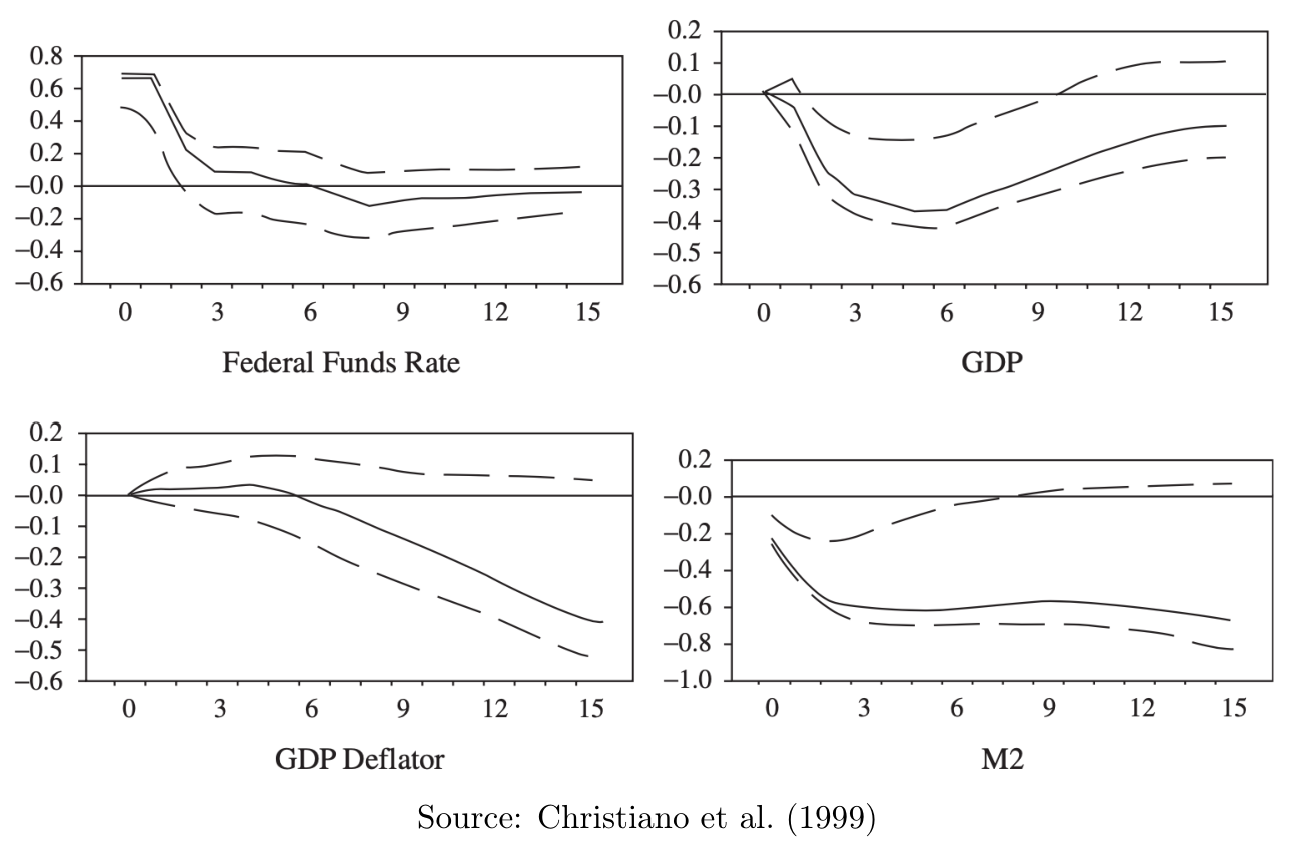
\includegraphics[width=0.8\textwidth]{figures/christiano1999.png}
    \caption{Estimated Dynamic Response to a Monetary Policy Shock (Quarterly)}
    \label{fig:christiano1999}
\end{figure}

\subsection{Criticisms of the VAR approach}

\begin{itemize}
    \item \textbf{Price Puzzle:} Observations show that after a contractionary policy shock, such as an increase in the Federal Funds Rate, 
    the price level tends to rise, which contradicts typical economic expectations. This phenomenon, known as the 'price puzzle,' 
    can be addressed by incorporating oil or commodity prices in the VAR system, 
    which are critical inflation-sensitive indicators that a standard VAR might omit.

    \item \textbf{Lack of Forward-Looking Variables:}\footnote{Most, if not all,
    of what one thinks of in terms of policy and policy design represents the endogenous response of policy
    to the economy, and “most variation in monetary policy instruments is accounted for by responses of
    policy to the state of the economy, not by random disturbances to policy”. (Sims and Zha 1998 \cite{sims1998bayesian})} 
    Many VAR models do not include forward-looking variables, 
    which are crucial as central banks often rely on forecasts of future economic conditions. 
    Without these, VARs might misattribute the impact of policy actions on subsequent economic outcomes.

    \item \textbf{Limitations of VAR Analysis:}
    \begin{itemize}
        \item VAR primarily captures the effects of monetary policy shocks -- unanticipated changes in policy which are not a response to the economic conditions.
        \item The majority of policy variations are endogenous, responding predictively to economic states rather than as exogenous shocks. 
        This is often not captured well by VAR.
        \item If monetary policy is seen solely as a feedback rule responding to the economy (with no exogenous shocks), 
        VAR could inaccurately suggest that monetary policy does not influence economic outcomes.
    \end{itemize}
    
    \item \textbf{Importance of Policy Response:} Despite VAR limitations, it's crucial to recognize that monetary policy's role is significant, 
    especially how the economy responds to non-policy shocks which may be strongly influenced by the nature of policy adjustments.

    \item \textbf{Relation to Macroeconomic Theory:} These points highlight concerns similar to those raised by the Lucas Critique about the limitations 
    of traditional econometric approaches in capturing the dynamic interplay between policy and economic outcomes.
\end{itemize}


Notably, as stated by Galí (2015\cite{gali2015monetary}), the RBC model had little relevance for the analysis of macroeconomic policy. We could add
monetary policy - as was done by papers such as Cooley and Hansen (1989\cite{cooley1989inflation}) - 
but, in the absence of any price or wage frictions, it would have no real effects.

To allow for a realistic model of business cycles and monetary policy, we need
a framework in which prices don't simply follow the money supply, and nominal interest rates and
inflation don't just move together one-for-one.

\begin{itemize}
    \item Outcome from this program is the “New Keynesian
    Synthesis”: combine RBC models with price rigidities.
    \item Money is non-neutral in the short run (Keynesian
    element), and neutral in the long run (classical element).
\end{itemize}

\section{The Monetary Transmission Mechanism}

Monetary policy should be a demand shock: loose MP should
stimulate demand through increased consumption and
investment.

We'll look into three questions and rech out to the New Keynesian model:
\begin{itemize}
    \item What determines demand (consumption/investment)?
    \item What is monetary policy exactly?
    \item The role of nominal rigidities.
\end{itemize}

\subsection{Households and nominal assets}

Nominal assets are bonds $B_t$ which pay interest at nominal rate $i_t$.
Ignore the labor-leisure choice, the households maximize:
\begin{align*}
    \max & \quad \mathbb{E}_t \sum_{i=0}^{\infty}U(C_{t+i} )\\
    \text{s.t.} & \quad P_{t+i}C_{t+i} + P_{t+i}K_{t+i+1} + B_{t+i+1} = W_{t+i}L + P_{t+i}(1+r_{t+i})K_{t+i} + (1+i_{t+i})B_{t+i} 
\end{align*}
where $W$ is the nominal wage, $P$ is the price of cunsumption goods,
$r_{t+i}$ is the rental rate of capital net of depreciation.

Define the Lagrangian:
\begin{align*}
    \mathcal{L} =\mathbb{E}_t\sum_{i=0}^{\infty} & \left[ U(C_{t+i} ) + \lambda_{t+i} \left( W_{t+i}L + P_{t+i}(1+r_{t+i})K_{t+i} + (1+i_{t+i})B_{t+i} \right. \right. \\ 
    &- \left. \left. P_{t+i}C_{t+i} - P_{t+i}K_{t+i+1} - B_{t+i+1} \right) \right]
\end{align*}

The FOCs are:
\begin{align*}
    U^{\prime} (C_{t+i} ) &= \mathbb{E}_t P_{t+i}\lambda_{t+i}  \\
    P_{t+i}\lambda_{t+i} &= \mathbb{E}_t \lambda_{t+i+1} P_{t+i+1} (1+r_{t+i+1}) \\
    \lambda_{t+i} &= \mathbb{E}_t \lambda_{t+i+1} (1+r_{t+i+1})
\end{align*}
Combining the first two, we get the standard Euler equation:
\[
    U^{\prime} (C_{t} ) = \mathbb{E}_t \left(U^{\prime} (C_{t+1} ) (1+r_{t+1})\right)
\]
Combine the first and the third:
\[
    U^{\prime} (C_{t} ) = \mathbb{E}_t \left(\frac{1+i_{t+1}}{1+\pi_{t+1}} U^{\prime} (C_{t+1} )\right)
\]
where inflation $\pi = \frac{P_{t+1} - P_t}{P_t}$.
\begin{align*}
    U^{\prime} (C_{t} ) &= \mathbb{E}_t \left(\frac{1+i_{t+1}}{1+\pi_{t+1}} U^{\prime} (C_{t+1} )\right) \\
    U^{\prime} (C_{t} ) &= \mathbb{E}_t \left((1+r_{t+1}) U^{\prime} (C_{t+1} )\right)
\end{align*}
 
\begin{itemize}
    \item What matters for the intertemporal consumption decision is
    the real interest rate, not the nominal interest rate.
    \item The FOC are necessary conditions for having both positive $B$
    and positive $K$. By the two equations above, we get:
    \[1+r_{t+1} = \frac{1+i_{t+1}}{1+\pi_{t+1}}. \]
    So, the \textcolor{red}{real return(interest rate)} of a nominal asset
    with \textcolor{red}{nominal interest rate} $1+i_{t+1} $ is: $\frac{1+i_{t+1} }{1+\pi_{t+1}}$.
    % \item This is the Fisher equation.
\end{itemize}

\begin{corollary}[Fisher equation]
    \ 

    It's the relationship between asset returns that has to hold 
    so that the household is willing to hold positive amounts 
    of these assets in their portfolio (or: if you allow negative 
    holdings, to clear asset markets).
    
    This relationship between the real and nominal rates of interest is called the Fisher relationship, 
    after Irving Fisher(1896)

    When households are risk-neutral, the FOCs become:
    \[\mathbb{E}_t (1+r_{t+1}) = \mathbb{E}_t \left(\frac{1+i_{t+1}}{1+\pi_{t+1}}\right) \]
    In a deterministic world, there's no $E$, which is often approxima.

    If we note that $(1+x)(1+y) \approx 1+x+y$, we can write the Fisher equation as:
    \[r_{t+1} \approx i_{t+1} - \pi_{t+1} \]
\end{corollary}

\subsection{Firms}
The firms would like to maximize profits, with perfect competition adn frictionless factor markets:
\[MPK = r\]
Again, \textit{real interest rate matters}. 

\textbf{Conclusion:} 
\underline{If monetary policy should affect demand, the real interest rate is the key price in the economy.}



\section{The tools of monetary policy}
So, in order to stimulate demand, the central bank needs to change the real interest rate.

\subsection*{How?}

\begin{itemize}
    \item Change the money supply, with demand curve, this would implement a particular nominal interest rate.
    \item Change the nominal interest rate directly.
\end{itemize}

\begin{tikzpicture}[
    node distance=1.5cm,
    block/.style={
        rectangle,
        draw,
        fill=blue!20,
        text width=5cm,
        text centered,
        rounded corners,
        minimum height=1cm
    },
    arrow/.style={
        thick,
        ->,
        >=Stealth
    }
]

% Nodes
\node (centralbank) [block] {Central Bank};

% First branch
\node (nominalrate1) [block, below left=of centralbank, xshift=2cm, yshift=-1cm] {Nominal interest rate i};

% Second branch
\node (nominalrate2) [block, below right=of centralbank, xshift=-2cm, yshift=-1cm] {Nominal interest rate i};

% Combined branch
\node (realrate) [block, below=of centralbank, yshift=-3cm] {Real interest rate r};
\node (consumption) [block, below=of realrate] {Consumption, Investment};
\node (output) [block, below=of consumption] {Output};

% Arrows for the first branch
\draw [arrow] (centralbank) -- (nominalrate1) node[midway, left, text width=4cm, align=left] {Sets and implements interest rate target};
\draw [arrow] (nominalrate1) -- (realrate) node[midway, left] {Nominal rigidities (?)};

% Arrows for the second branch
\draw [arrow] (centralbank) -- (nominalrate2) node[midway, right, text width=7cm, align=left] {Sets money supply, given a money demand curve and money market clearing we get a nominal interest rate i};
\draw [arrow] (nominalrate2) -- (realrate) node[midway, right] {Nominal rigidities (?)};

% Arrows for the combined branch
\draw [arrow] (realrate) -- (consumption) node[midway, left] {Intertemporal Euler equation};
\draw [arrow] (consumption) -- (output) node[midway, left] {Given an output supply curve};

\end{tikzpicture}

\subsection{Money supply-demand equilibrium}

Originally, the money market equilibrium is the IS-LM curve, if 
\begin{figure}[!htbp]
    \centering
    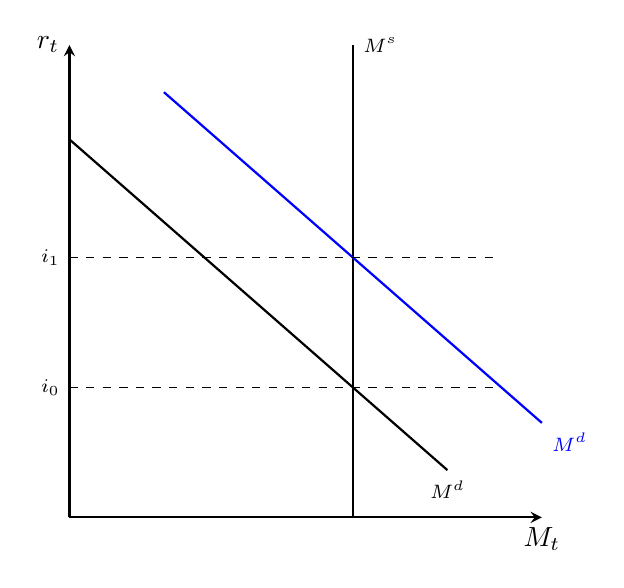
\begin{tikzpicture}[>=stealth, scale=1.2]

        % Axes
        \draw[thick,->] (0,0) -- (5,0) node[below] {$M_t$};
        \draw[thick,->] (0,0) -- (0,5) node[left] {$r_t$};
        
        % Vertical line (Money supply)
        \draw[thick] (3,0) -- (3,5) node[right] {\scriptsize $M^s$};
        
        % Downward sloping demand curve (initial)
        \draw[thick] (0,4) -- (4,0.5) node[below] {\scriptsize $M^d$};
        
        % Downward sloping demand curve (shifted)
        \draw[thick,blue] (1,4.5) -- (5,1) node[below right] {\textcolor{blue}{\scriptsize $M^d$}};
        
        % Dashed lines for equilibrium points
        \draw[dashed] (0,2.75) -- (4.5,2.75) node[pos=0,left] {\scriptsize $i_1$};
        \draw[dashed] (0,1.375) -- (4.5,1.375) node[pos=0,left] {\scriptsize $i_0$};
    \end{tikzpicture}
\end{figure}

If we have a interest rate target and implement particular interest rate,

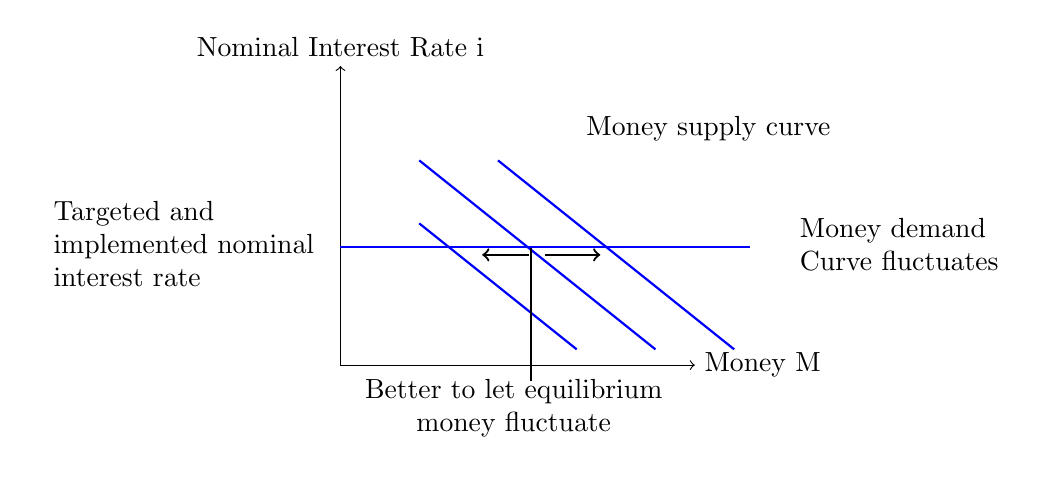
\begin{tikzpicture}[scale=1]
    \draw[->] (0,0) -- (4.5,0) node[right] {Money M};
    \draw[->] (0,0) -- (0,3.8) node[above] {Nominal Interest Rate i};
    
    % Money demand curves
    \draw[blue, thick] (1,2.6) -- (4,0.2);
    \draw[blue, thick] (2,2.6) -- (5,0.2);
    \draw[blue, thick] (1,1.8) -- (3,0.2);
    
    % % Money supply curve (vertical line)
    \draw[black, thick] (2.42,1.5) -- (2.42,-0.2);
    
    % Horizontal line for targeted interest rate
    \draw[blue, thick] (0,1.5) -- (5.2,1.5);
    
    % Arrows showing fluctuation
    \draw[->, thick] (2.4,1.4) -- (1.8,1.4);
    \draw[->, thick] (2.6,1.4) -- (3.3,1.4);
    
    % Labels
    \node[left] at (0,1.5) {\begin{tabular}{l}Targeted and\\implemented nominal\\interest rate\end{tabular}};
    \node[below] at (2.2,0) {\begin{tabular}{c}Better to let equilibrium\\money fluctuate\end{tabular}};
    \node[right] at (3,3) {Money supply curve};
    \node[right] at (5.5,1.5) {\begin{tabular}{l}Money demand\\Curve fluctuates\end{tabular}};
\end{tikzpicture}

\section{A model of the interbank market}

Then, we first build a model for interbank market,
\begin{itemize}
    \item Market participants: $n$ banks.
    \item Banks hold reserves at the central bank.
    \item Reserves are used for settling transfers between banks arising from the payment system.
    \item Banks are unsure of the transfers htey will need to make.
    \item Banks can borrow reserves from one another in the interbank market,
    but do not know how much reserve they'll require at the point they participate in the interbank market.
    \item Banks can also acquire reserves through the repo (repurchase
    agreement) market. The central bank can be a participant in
    this market.
\end{itemize}

\begin{note}
    \ 

    $B_j$ = reserves of bank $j$ at beginning-of-period.(after previous debts settles) \\
    $I_j$ = net borrowing in the interbank market (negative for
    lending) by bank $j$. \\
    $P_j$ = net bond repos(sales and repurchases) by bank $j$. \\
    $T_j$ = net payment bank $j$ make to other banks. \\
    $R_j$ = balance of bank $j$ at end-of-period. \\
    Accounting: $R_j = B_j + I_j + P_j - T_j$.
\end{note}

\subsection{Interbank market and repo market}
\textbf{Interbank market:}
\begin{itemize}
    \item Uncollateralized loans between banks.(potentially risky)
    \item Interest rate $i$.
\end{itemize}

\textbf{Repo market:}
\begin{itemize}
    \item Sell bond now and agree to repurchase later.
    \item Effectively a collaboratized loan, so risk-free if collateral is good.
\end{itemize}

\begin{note}[Central bank facilities]
    \ 

    \textbf{Deposit Facility:} Centrla bank offers an interest rate of $i_d$ on deposit balances in banks' account at the end of time period.

    \textbf{Borrowing facility:} Central bank charges an interest rate $i_b$ on negative balances in banks' accounts.
    \begin{itemize}
        \item Positive spread over deposit rate: $i_b > i_d$.
        \item Equivalent to an offer to make loans at the end of perios, with the load credited to the bank's account.
        \item Collateral required -- we should assune banks have enough collateral to use it.
    \end{itemize}
\end{note}

\subsection{Balance on account next period}

Reserve balance of bank $j$ at the end of period is:
\[
B^{\prime} _j = R_j - (1+i)(I_j + P_j) + \left\{\begin{matrix}
   i_d R_j & \text{if } R_j \geq 0\\
   i_b R_j & \text{if } R_j < 0
  \end{matrix}\right.
\]
Since $R_j = B_j + I_j + P_j - T_j$, we have:
\[
B^{\prime} _j = B_j - T_j - i(I_j + P_j) + \left\{\begin{matrix}
   i_d (B_j + I_j + P_j - T_j) & \text{if } B_j + I_j + P_j - T_j \geq 0\\
   i_b (B_j + I_j + P_j - T_j) & \text{if } B_j + I_j + P_j - T_j < 0
  \end{matrix}\right.
\]

Assume banks are risk-neutral, and they aim to maximize their next period expected balance $\mathbb{E}(B^{\prime}_j)$.
Choice variabls are: interbank transaction $I_j$, repo market transaction $P_j$.
\begin{align*}
    \mathbb{E}(B^{\prime}_j) = B_j - i(I_j + P_j) &+ i_d \int_{-\infty}^{B_j + I_j + P_j} (B_j + I_j + P_j - T_j) dF(T_j) \\
    &+ i_b \int_{B_j + I_j + P_j}^{\infty} (B_j + I_j + P_j - T_j) dF(T_j)
\end{align*}
The FOCs are:
\begin{align*}
    \frac{\partial \mathbb{E}(B^{\prime}_j)}{\partial I_j} &= 0 \\
    \frac{\partial \mathbb{E}(B^{\prime}_j)}{\partial P_j} &= 0
\end{align*}

Two equations lead to the same equation, so we only consider one of them.
\begin{theorem}[Leibniz Rule]
    \ 
    
    Let $f(x, t)$ be a function such that both $f(x, t)$ and 
    its partial derivative $f_x(x, t)$ are continuous in $t$ and 
    $x$ in some region of the $xt$-plane, 
    including $a(x) \leq t \leq b(x)$, $x_0 \leq x \leq x_1$. 
    Also suppose that the functions $a(x)$ and $b(x)$ are both continuous 
    and both have continuous derivatives for $x_0 \leq x \leq x_1$. 
    Then, for $x_0 \leq x \leq x_1$,
    \[
    \frac{d}{dx} \left( \int_{a(x)}^{b(x)} f(x, t) \, dt \right) = f(x, b(x)) \cdot \frac{d}{dx} b(x) - f(x, a(x)) \cdot \frac{d}{dx} a(x) + \int_{a(x)}^{b(x)} \frac{\partial}{\partial x} f(x, t) \, dt.
    \]
\end{theorem}

Use the Leibniz rule:
\begin{align*}
    & \frac{\partial}{\partial I_j} \int_{-\infty}^{B_j + I_j + P_j} (B_j + I_j + P_j - T_j) dF(T_j) \\
    &= \int_{-\infty}^{B_j + I_j + P_j} f(T_j)d T_j + \left((B_j + I_j + P_j) - (B_j + I_j + P_j)\right)f(B_j + I_j + P_j) \\
    &= F(B_j + I_j + P_j) 
\end{align*}
Similarly,
\begin{align*}
    & \frac{\partial}{\partial I_j} \int_{B_j + I_j + P_j}^{\infty} (B_j + I_j + P_j - T_j) dF(T_j) \\
    &= 1 - F(B_j + I_j + P_j)
\end{align*}
Hence, the FOC reduces to:
\[
-i + i_d F(B_j + I_j + P_j) + i_b (1 - F(B_j + I_j + P_j)) = 0
\]
Equivalently,
\[
(i - i_d)F(B_j + I_j + P_j) = (i_b - i)(1 - F(B_j + I_j + P_j))
\]
The optimal demand for interbank and repo lending is characterized by the equation: 
\[
F(B_j + I_j + P_j) = \frac{i_b - i}{i_b - i_d}
\]
Since we know that $0 \leq F(B_j + I_j + P_j) \leq 1$, the FOC implies that:
\[i_d \leq i \leq i_b.\]
So, the interest rate $i$ lies in the channel $[i_d, i_b]$.
\begin{note}
    \ 

    No one would lend at an interest rate lower than what you get from the central bank,
    and no one would borrow at an interest rate higher than what you have to pay to the central bank.
\end{note}

Since $F$ is increasing, there is a negative relationship between $i \text{ and } I_j + P_j.$

\subsection{Aggregation and market clearing}
\begin{align*}
    B &= \sum_{j=1}^{n}B_j (\text{Aggregate beginning-of-period balances})\\
    P &= \sum_{j=1}^{n}P_j (\text{Aggregate end-of-period balances})\\
    T &= \sum_{j=1}^{n}T_j = 0 (\text{payments between banks cancel out})  \\
    R &= \sum_{j=1}^{n}R_j
\end{align*}

Since $R_j = B_j + I_j + P_j - T_j$, we have $R = B+P$ in the aggregate.

Since $B_j + I_j + P_j$ is the same for all banks: $B_j + I_j + P_j = \frac{R}{n}$.

\subsection{Equilibrium interbank interest rate}
\begin{align*}
    F\left(\frac{R}{n}\right) &= \frac{i_b - i}{i_b - i_d} \\
    \frac{R}{n} &= F^{-1}\left(\frac{i_b - i}{i_b - i_d}\right) \\
    i &= i_d + \frac{i_b - i_d}{n} \int_{-\infty}^{F^{-1}\left(\frac{i_b - i}{i_b - i_d}\right)} x dF(x)
\end{align*}

THe central bank directly controls:
\begin{itemize}
    \item $i_d$ and $i_b$.
    \item Open market operations $P$.
\end{itemize}
Indirectly determinems
\begin{itemize}
    \item Interbank and repo rate $i$.
    \item Total end-of-period reserves $R = B+P$.
\end{itemize}

\subsection{Interbank market with channel system}

\begin{itemize}
    \item \textbf{Demand:} Equation $F\left(\frac{R}{n}\right) = \frac{i_b - i}{i_{b-i_d}}$, giving a negative relationship between $i$ and $R$.
    \item \textbf{Supply:} Central bank sets $R = B+P$ by open market operations.
\end{itemize}

If we hold all other policy instruments constant,
\begin{itemize}
    \item An increase in total reserves $R$ will shift supply curve to the right, decreasing $i$.
    \item An increase in $i_d$ will shift demand curve upward, increasing $i$.
    \item An increase in $i_b$ will shift demand curve upward, increasing $i$.
\end{itemize}

\begin{figure}[!htbp]
    \centering
    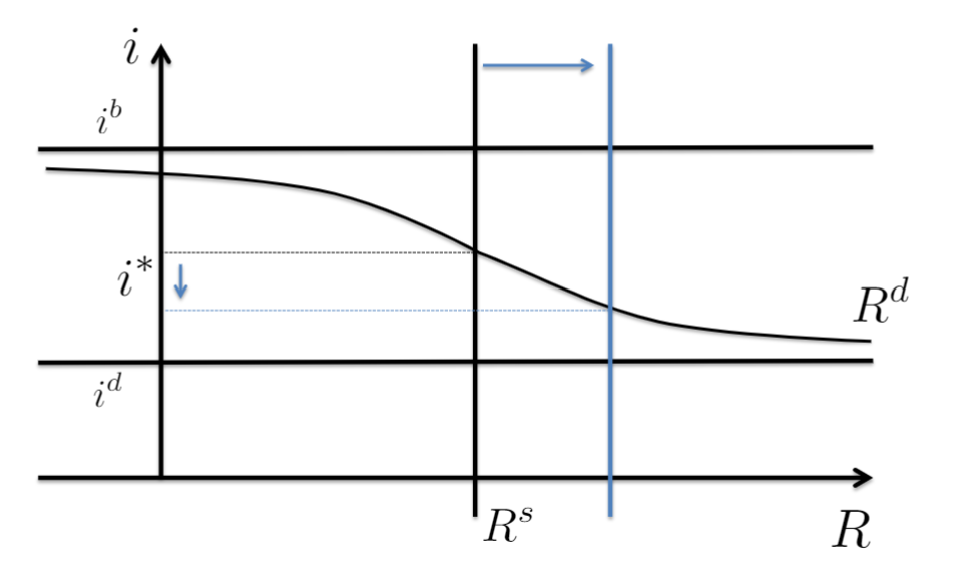
\includegraphics[width=0.8\textwidth]{figures/PS(3).png}
    \caption{Increasing Open Market operations}
\end{figure}

\begin{figure}
    \centering
    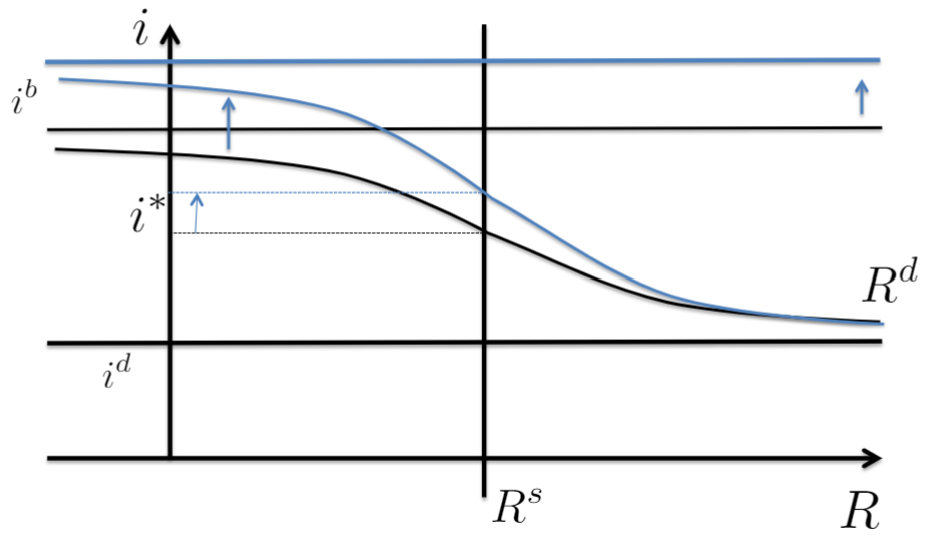
\includegraphics[width=0.8\textwidth]{figures/PS(3)-2.png}
    \caption{Increasing $i_b$ or $i_d$(similar)}
\end{figure}

Then, if the central bank would like to increase $i$ by $x$, while both $i_b$ and $i_d$ increase by $x$,
no new open market operations are needed.

\begin{note}
    \ 

    A narrow channel has advantages:
    \begin{itemize}
        \item More precise control of $i$, less fluctuations.
        \item Less need for open market operations.
    \end{itemize}

    There'are also disadvantages, e.g. $i_b = i_b$:
    \begin{itemize}
        \item Trading in interbank market dries up.
        \item CB becomes the intermediary of all borrowing and lending between banks, hence it incurs the cost of monitoring credit-worthiness of banks. \textcolor{red}{It's not the central bank's job.}
    \end{itemize}
\end{note}

\subsection{Interest rate maturity}

\begin{question}
    \

    How does this affect medium- and long-term interest rates? \\
    How are interest rates of different maturities related?
\end{question}

\begin{eg}
    \ 

    Imagine an investor invest for 2 years:
    \begin{itemize}
        \item Buy a 2-year bond, keep until it matures: \[\text{return} = 1 + i_t^{(2y)}\]
        \item Buy a 1-year bond, then buy another 1-year bond: \[\text{return} = (1+i_t^{(1y)})(1+i_{t+1}^{(1y)})\]    
    \end{itemize}

    \textbf{Expectations Hypothesis:} Expectations of these two returns should be the same:
    \[i_t^{(2y)} = \mathbb{E}_t (1 + i_t^{(1y)})(1 + i_{t+1}^{(1y)}).\]

    This should hold exactly if agents are risk-neutral. With risk aversion, one would adjust the expected retuen for riskiness.

    But, still, the current long-term rate is determined by the current short-term rate and the expected future short-term rates.
    \begin{note}
        \ 

        CB can use announcements of future policies to affect long-term rates.
    \end{note}
\end{eg}
